\documentclass[Thesis.tex]{subfiles}
\begin{document}
\chapter{Monte Carlo Methods}
\label{chp:monte-carlo}

In \autoref{chp:variational-monte-carlo} we found that we needed a way to
sample system configurations $\vX$ from the probability distribution  described
by the wave function. We needed this as a means to evaluate integrals. Specifically, we needed to evaluate the expectation value of the Hamiltonian w.r.t. a given wave function $\psialpha$:

\begin{align}
    \expval{\hat H} &= \frac{\expval{\hat H}{\psialpha}}{\braket{\psialpha}} = \int\dd{\vX} P_{\psi_{\valpha}} (\vX) E_L(\vX)\label{eq:chp-mc-anon-1}\\
    &\approx \frac{1}{N} \sum_{i = 1}^N E_L(\vX_i)
    \qq{where} \vb X_i\sim P_{\psi_{\valpha}}
\end{align}
where $N$ is set sufficiently large to satisfy the required accuracy. Due to
the central nature of this method, we will start by a proper presentation of
Monte Carlo Integration as it is used here, followed the details of how to
obtain the samples we need.

\section{Monte Carlo Integration}

Monte Carlo Integration (MCI) is a general technique for numeric evaluation of any arbitrary integral. In general it concerns evaluating any multidimensional definite integral, written as

\begin{align}
    I = \idotsint_\sigma\dd{\vx} f(\vx)
\end{align}
where $\sigma$ denotes a subset of $\mathbb{R}^m$, with a $m$-dimensional volume given by
\begin{align}
    V = \idotsint_\sigma\dd{\vx}
\end{align}
In its simplest form, MCI samples $N$ \emph{uniformly} distributed points
$\vx_1,\dots,\vx_N$ from $\sigma$, and uses a Riemann sum formulation of the integral $I$:
\begin{align}
    I = \lim_{N\to\infty} M_N \defeq \lim_{N\to\infty}\sum_{i=1}^N f(\vx_i) \frac{V}{N} = V\expval{f(\vx)}_\sigma
\end{align}
where $\expval{\cdot}_\sigma$ denotes the expectation value over all points in $\sigma$. For finite $N$ we may obtain estimates of the error we make in approximating the integral. First, we estimate the variance of the integrand:
\begin{align}
    \Var[f(\vx)] = \sigma^2_N = \frac{1}{N-1} \sum_{i=1}^Nf(\vx_i)
\end{align}
It then follows, by the properties of variance,
\begin{align}
    \Var[M_N] = \Var\qty[ \frac{V}{N} \sum_{i=1}^Nf(\vx_i)] = \frac{V^2}{N^2}\sum_{i=1}^N\Var[f(\vx_i)] = \frac{V^2\sigma^2_N}{N}
\end{align}
\begin{align}
    \implies \Std[M_N] = \sqrt{\Var[M_N]} = \frac{V\sigma_N}{\sqrt N}
\end{align}
This tells us that the expected statistical error we make goes like
$\mathcal{O}(1 / \sqrt N)$, and depends linearly on the size of the volume.
This illustrates both the advantage, and disadvantage of Monte Carlo
integration compared to other, deterministic integration methods. Its advantage
is its simple dependency on the volume, and its independence from the
particular number of dimensions in the integral. Other methods tend to depend
exponentially on the dimensionality, and as such MCI is often the best choice
for multidimensional integrals. Its disadvantage is the relatively slow
convergence rate, which is asymptotically much worse than other
approaches~\cite{Numerical-Recipes-Press-et-al}.

\subsection{Importance Sampling}

In some suitable cases we can improve quite dramatically on the simple,
straightforward approach presented above. To illustrate this, say we
would like to evaluate the following integral:

\begin{align}
    \label{eq:mci-importance-example-func}
    I = \intfy\dd{x}f(x)=\intfy\dd{x} \frac{\exp{-\flatfrac{x^2}{2} }}{\sqrt{2\pi \qty(1 +x^2)}}  = \num{0.78964}.
\end{align}

\begin{figure}
    \centering
    \resizebox{0.8\linewidth}{!}{%
    \begin{tikzpicture}
        \begin{axis}[every axis plot post/.append style={
                mark=none,domain=-5:5,samples=50,smooth}, % All plots: from -2:2, 50 samples, smooth, no marks
            axis x line=bottom, % no box around the plot, only x and y axis
            axis y line=left,
            enlargelimits=upper] % extend the axes a bit to the right and top
            \addplot[semithick, color0] {1/(sqrt(2*pi))*exp(-(x^2)/2)*(1+x^2)^(-0.5)};
            \addplot[semithick, color1] {1/(sqrt(2*pi))*exp(-(x^2)/2)};
            \addlegendentry{$f(x)$}
            \addlegendentry{$\mathcal{N}(0, 1)$}
        \end{axis}
    \end{tikzpicture}
    }
    \caption{\label{fig:mci-importance-example-func-plot}Plot of the function in \autoref{eq:mci-importance-example-func}}
\end{figure}
The integrand is plotted in \autoref{fig:mci-importance-example-func-plot}, and
the observant reader might recognise this as the product of a normal
distribution and a Student-t distribution. The correct value for the integral
is also given, so we have a reference for the results.

For comparison, lets start with the straightforward approach from before.
Because the integral goes to infinity the "volume" $V$ would not be well
defined, and we are forced to truncate the region manually. From looking at the
graph in \autoref{fig:mci-importance-example-func-plot} we may say that $x\in
[-5, 5]$ should account for the vast majority of the total integral. That means
we use the following estimate:

\begin{align}
    \label{eq:chp-mc-anon-2}
    I\approx \frac{10}{N}\sum_{i=1}^Nf(x_i)\qq{where} x_i\sim\text{Uniform}(-5, 5)
\end{align}

The main issue with this approach is that 1) we need to truncate the integral
manually and 2) now matter where we place the box boundaries we will tend to
sample a lot of $x_i$'s in areas where $f$ gives very small contributions to
the integral. Ideally we would like our sample points to be distributed as
closely as possible to $f$, in order to capture as much information as we can.
This is the idea of importance sampling. Instead of using the uniform
distribution for sampling, we use some probability distribution which more
closely resembles the integrand, call it $g(x)$. Formally we then restate the integral as follows:

\begin{align}
    I = \intfy\dd{x}f(x) = \intfy\dd{x} \frac{f(x)}{g(x)} g(x)
\end{align}
This can be interpreted as the expectation of $z(x)=\flatfrac{f(x)}{g(x)}$ for $x$'s drawn from $g$, and so the corresponding estimation is then:

\begin{align}
    I \approx \frac{1}{N} \sum_{i=1}^N \frac{f(x_i)}{g(x_i)} \qq{where} x_i\sim g
\end{align}
Setting $g = \text{Uniform}(-5, 5)$ recovers \autoref{eq:chp-mc-anon-2}, so this is simply the natural generalization of the standard approach for an arbitrary distribution function $g$.


Going back to the example, we should now chose a distribution function that
closely resembles the integrand, while still being simple to sample from. In
this (contrived) example, a natural choice is to use the standard normal
distribution, $g = \mathcal{N}(0, 1)$. In
\autoref{fig:mci-importance-example-func-plot} we can see how $g(x)$ is
enclosing $f(x)$ much more tightly than any rectangular box might hope to.

\begin{figure}
   \centering
    \resizebox{\linewidth}{!}{%
        % This file was created by matplotlib2tikz v0.7.4.
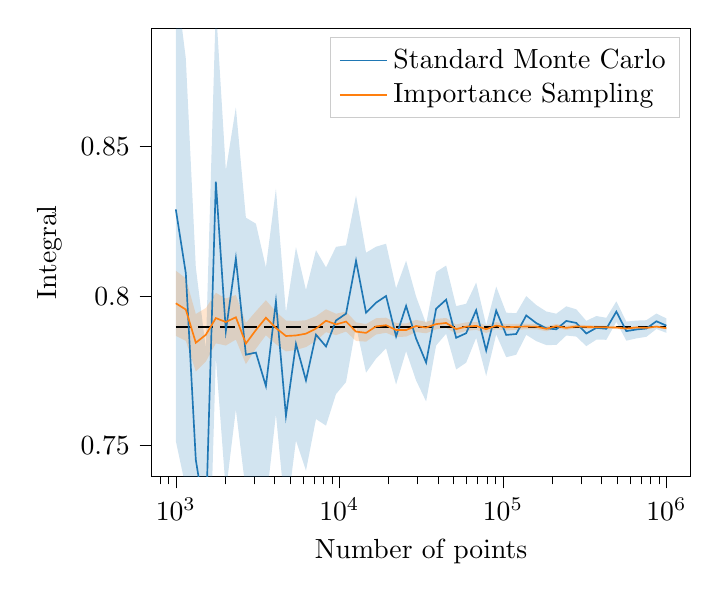
\begin{tikzpicture}

\definecolor{color0}{rgb}{0.12156862745098,0.466666666666667,0.705882352941177}
\definecolor{color1}{rgb}{1,0.498039215686275,0.0549019607843137}

\begin{axis}[
legend cell align={left},
legend style={draw=white!80.0!black},
log basis x={10},
tick align=outside,
tick pos=left,
x grid style={white!69.01960784313725!black},
xlabel={Number of points},
xmin=707.945784384138, xmax=1412537.54462276,
xmode=log,
xtick style={color=black},
y grid style={white!69.01960784313725!black},
ylabel={Integral},
ymin=0.73964, ymax=0.88964,
ytick style={color=black}
]
\path [fill=color0, fill opacity=0.2]
(axis cs:1000,0.906505519198725)
--(axis cs:1000,0.751532172525837)
--(axis cs:1151,0.735831543753176)
--(axis cs:1325,0.680849621063098)
--(axis cs:1526,0.66635670415917)
--(axis cs:1757,0.779382816946574)
--(axis cs:2023,0.734566699673617)
--(axis cs:2329,0.762035463989511)
--(axis cs:2682,0.734565832804202)
--(axis cs:3088,0.73798169568494)
--(axis cs:3556,0.730217784390541)
--(axis cs:4094,0.760469759098198)
--(axis cs:4714,0.725360612203807)
--(axis cs:5428,0.751700043683699)
--(axis cs:6250,0.741602925670416)
--(axis cs:7196,0.758867234301727)
--(axis cs:8286,0.756687693428198)
--(axis cs:9540,0.767228880540759)
--(axis cs:10985,0.771229626136113)
--(axis cs:12648,0.790012094541718)
--(axis cs:14563,0.774391523089762)
--(axis cs:16768,0.77909942060995)
--(axis cs:19306,0.782536739216005)
--(axis cs:22229,0.770428521449884)
--(axis cs:25595,0.781574784789273)
--(axis cs:29470,0.771759717058446)
--(axis cs:33932,0.764776709236966)
--(axis cs:39069,0.783487769922224)
--(axis cs:44984,0.787414355694207)
--(axis cs:51794,0.775475553467901)
--(axis cs:59636,0.777740489465899)
--(axis cs:68664,0.786049955378521)
--(axis cs:79060,0.773275873950683)
--(axis cs:91029,0.787160195206047)
--(axis cs:104811,0.779567528991012)
--(axis cs:120679,0.780390365577674)
--(axis cs:138949,0.787053593717609)
--(axis cs:159985,0.784957670264303)
--(axis cs:184206,0.783635621994808)
--(axis cs:212095,0.783663303380307)
--(axis cs:244205,0.786824569813399)
--(axis cs:281176,0.786472339541122)
--(axis cs:323745,0.783270774763061)
--(axis cs:372759,0.785431295025521)
--(axis cs:429193,0.785403139227959)
--(axis cs:494171,0.79137576492629)
--(axis cs:568986,0.785095481165753)
--(axis cs:655128,0.785862960669846)
--(axis cs:754312,0.786388810526214)
--(axis cs:868511,0.789001256366245)
--(axis cs:1000000,0.78771906388357)
--(axis cs:1000000,0.792542831612807)
--(axis cs:1000000,0.792542831612807)
--(axis cs:868511,0.794181220859291)
--(axis cs:754312,0.791942882951014)
--(axis cs:655128,0.791820110680025)
--(axis cs:568986,0.791487504496917)
--(axis cs:494171,0.798260611327551)
--(axis cs:429193,0.792759708194515)
--(axis cs:372759,0.793337949884088)
--(axis cs:323745,0.791729598374579)
--(axis cs:281176,0.795583619643708)
--(axis cs:244205,0.796589010550667)
--(axis cs:212095,0.79412837031455)
--(axis cs:184206,0.794870279758202)
--(axis cs:159985,0.79701634187077)
--(axis cs:138949,0.800016332107068)
--(axis cs:120679,0.794272570875621)
--(axis cs:104811,0.794468511086953)
--(axis cs:91029,0.803200188932203)
--(axis cs:79060,0.790355947691124)
--(axis cs:68664,0.804549926843196)
--(axis cs:59636,0.797454867544406)
--(axis cs:51794,0.796653185040259)
--(axis cs:44984,0.810244363594127)
--(axis cs:39069,0.808073653372737)
--(axis cs:33932,0.790777573023198)
--(axis cs:29470,0.799841366593076)
--(axis cs:25595,0.811867722605131)
--(axis cs:22229,0.802618543013231)
--(axis cs:19306,0.817530506209257)
--(axis cs:16768,0.816541914366059)
--(axis cs:14563,0.814542168015885)
--(axis cs:12648,0.833651170719542)
--(axis cs:10985,0.817018107595682)
--(axis cs:9540,0.816494291003619)
--(axis cs:8286,0.809610747560487)
--(axis cs:7196,0.815367040536989)
--(axis cs:6250,0.802025469808376)
--(axis cs:5428,0.816380403842103)
--(axis cs:4714,0.79455756611557)
--(axis cs:4094,0.83595037286634)
--(axis cs:3556,0.809617017360876)
--(axis cs:3088,0.824249680097279)
--(axis cs:2682,0.826250438806259)
--(axis cs:2329,0.863177790933464)
--(axis cs:2023,0.842110084892558)
--(axis cs:1757,0.897157433940518)
--(axis cs:1526,0.782467186210373)
--(axis cs:1325,0.809627874200951)
--(axis cs:1151,0.879506727836154)
--(axis cs:1000,0.906505519198725)
--cycle;

\path [fill=color1, fill opacity=0.2]
(axis cs:1000,0.808499519570512)
--(axis cs:1000,0.786713211329766)
--(axis cs:1151,0.785042642420524)
--(axis cs:1325,0.774788109289872)
--(axis cs:1526,0.778119575109797)
--(axis cs:1757,0.784198893001299)
--(axis cs:2023,0.783474555689343)
--(axis cs:2329,0.785454412684189)
--(axis cs:2682,0.777230046137711)
--(axis cs:3088,0.782391418189927)
--(axis cs:3556,0.786909552632689)
--(axis cs:4094,0.783902603834432)
--(axis cs:4714,0.781495885789912)
--(axis cs:5428,0.781995739197111)
--(axis cs:6250,0.782947354122917)
--(axis cs:7196,0.785013543050367)
--(axis cs:8286,0.787948023436544)
--(axis cs:9540,0.786939718155325)
--(axis cs:10985,0.78813969801641)
--(axis cs:12648,0.785009178650894)
--(axis cs:14563,0.784773520932163)
--(axis cs:16768,0.787148101226365)
--(axis cs:19306,0.787741557498044)
--(axis cs:22229,0.786316999755659)
--(axis cs:25595,0.786450329615228)
--(axis cs:29470,0.787955851294709)
--(axis cs:33932,0.78757265986175)
--(axis cs:39069,0.788869680545658)
--(axis cs:44984,0.78938055958093)
--(axis cs:51794,0.787415451512896)
--(axis cs:59636,0.788357903529426)
--(axis cs:68664,0.788705910542103)
--(axis cs:79060,0.787681126030283)
--(axis cs:91029,0.78898051397606)
--(axis cs:104811,0.788492546402297)
--(axis cs:120679,0.788732894196601)
--(axis cs:138949,0.788892819560814)
--(axis cs:159985,0.788902704579644)
--(axis cs:184206,0.788249963966235)
--(axis cs:212095,0.789177671294473)
--(axis cs:244205,0.788671473735971)
--(axis cs:281176,0.789205696562338)
--(axis cs:323745,0.789094062911801)
--(axis cs:372759,0.789032879202963)
--(axis cs:429193,0.789047047758369)
--(axis cs:494171,0.789002100901894)
--(axis cs:568986,0.788704796739401)
--(axis cs:655128,0.789067389752803)
--(axis cs:754312,0.788974080074391)
--(axis cs:868511,0.78943145779477)
--(axis cs:1000000,0.788914352720739)
--(axis cs:1000000,0.789617741825269)
--(axis cs:1000000,0.789617741825269)
--(axis cs:868511,0.790185812364)
--(axis cs:754312,0.789784265247556)
--(axis cs:655128,0.789935551227239)
--(axis cs:568986,0.789637087545991)
--(axis cs:494171,0.790002016054565)
--(axis cs:429193,0.790120519045172)
--(axis cs:372759,0.790181903582851)
--(axis cs:323745,0.790329990198755)
--(axis cs:281176,0.790532034926843)
--(axis cs:244205,0.790094903469465)
--(axis cs:212095,0.790704776107281)
--(axis cs:184206,0.789891414252003)
--(axis cs:159985,0.790658336939786)
--(axis cs:138949,0.790774959557188)
--(axis cs:120679,0.790755694443077)
--(axis cs:104811,0.790661819627759)
--(axis cs:91029,0.791309731968405)
--(axis cs:79060,0.790182700029323)
--(axis cs:68664,0.791381769122267)
--(axis cs:59636,0.791238449252401)
--(axis cs:51794,0.790511201000009)
--(axis cs:44984,0.792681004890301)
--(axis cs:39069,0.792413735793226)
--(axis cs:33932,0.791381426805788)
--(axis cs:29470,0.79204983187053)
--(axis cs:25595,0.790859203245189)
--(axis cs:22229,0.79101619799564)
--(axis cs:19306,0.792788925820531)
--(axis cs:16768,0.792596552778913)
--(axis cs:14563,0.790644584700561)
--(axis cs:12648,0.791243995361164)
--(axis cs:10985,0.794832730416374)
--(axis cs:9540,0.794115920221445)
--(axis cs:8286,0.795606481910413)
--(axis cs:7196,0.793283271523529)
--(axis cs:6250,0.791946308583509)
--(axis cs:5428,0.79169137563027)
--(axis cs:4714,0.791830711268204)
--(axis cs:4094,0.794798753178707)
--(axis cs:3556,0.798644174762259)
--(axis cs:3088,0.794920715642714)
--(axis cs:2682,0.791056764105328)
--(axis cs:2329,0.800402702389645)
--(axis cs:2023,0.799215779199193)
--(axis cs:1757,0.801113437531119)
--(axis cs:1526,0.796022529704722)
--(axis cs:1325,0.794032465873107)
--(axis cs:1151,0.805985030304646)
--(axis cs:1000,0.808499519570512)
--cycle;

\path [draw=black, semithick, dash pattern=on 5.550000000000001pt off 2.4000000000000004pt]
(axis cs:1000,0.78964)
--(axis cs:1000000,0.78964);

\addplot [semithick, color0]
table {%
1000 0.829018845862281
1151 0.807669135794665
1325 0.745238747632025
1526 0.724411945184771
1757 0.838270125443546
2023 0.788338392283088
2329 0.812606627461488
2682 0.78040813580523
3088 0.781115687891109
3556 0.769917400875709
4094 0.798210065982269
4714 0.759959089159688
5428 0.784040223762901
6250 0.771814197739396
7196 0.787117137419358
8286 0.783149220494342
9540 0.791861585772189
10985 0.794123866865898
12648 0.81183163263063
14563 0.794466845552823
16768 0.797820667488005
19306 0.800033622712631
22229 0.786523532231558
25595 0.796721253697202
29470 0.785800541825761
33932 0.777777141130082
39069 0.795780711647481
44984 0.798829359644167
51794 0.78606436925408
59636 0.787597678505153
68664 0.795299941110859
79060 0.781815910820903
91029 0.795180192069125
104811 0.787018020038983
120679 0.787331468226647
138949 0.793534962912339
159985 0.790987006067536
184206 0.789252950876505
212095 0.788895836847429
244205 0.791706790182033
281176 0.791027979592415
323745 0.78750018656882
372759 0.789384622454805
429193 0.789081423711237
494171 0.794818188126921
568986 0.788291492831335
655128 0.788841535674935
754312 0.789165846738614
868511 0.791591238612768
1000000 0.790130947748189
};
\addlegendentry{Standard Monte Carlo}
\addplot [semithick, color1]
table {%
1000 0.797606365450139
1151 0.795513836362585
1325 0.784410287581489
1526 0.787071052407259
1757 0.792656165266209
2023 0.791345167444268
2329 0.792928557536917
2682 0.784143405121519
3088 0.788656066916321
3556 0.792776863697474
4094 0.78935067850657
4714 0.786663298529058
5428 0.78684355741369
6250 0.787446831353213
7196 0.789148407286948
8286 0.791777252673478
9540 0.790527819188385
10985 0.791486214216392
12648 0.788126587006029
14563 0.787709052816362
16768 0.789872327002639
19306 0.790265241659288
22229 0.788666598875649
25595 0.788654766430209
29470 0.790002841582619
33932 0.789477043333769
39069 0.790641708169442
44984 0.791030782235616
51794 0.788963326256453
59636 0.789798176390914
68664 0.790043839832185
79060 0.788931913029803
91029 0.790145122972232
104811 0.789577183015028
120679 0.789744294319839
138949 0.789833889559001
159985 0.789780520759715
184206 0.789070689109119
212095 0.789941223700877
244205 0.789383188602718
281176 0.789868865744591
323745 0.789712026555278
372759 0.789607391392907
429193 0.789583783401771
494171 0.78950205847823
568986 0.789170942142696
655128 0.789501470490021
754312 0.789379172660974
868511 0.789808635079385
1000000 0.789266047273004
};
\addlegendentry{Importance Sampling}
\end{axis}

\end{tikzpicture}
    }
    \caption{\label{fig:mci-importance-example-func-convergence}Convergence of
    the integral in \autoref{eq:mci-importance-example-func}, using regular
    Monte Carlo integration and Importance Sampling with $g = \mathcal{N}(0,
    1)$. The points indicate the approximated value of the integral for each
    particular experiment, and the shaded areas indicate the corresponding
    $\SI{95}{\percent}$ confidence intervals for the expected value. We see the
    latter displaying both greater accuracy and tighter confidence intervals.
    The source code for this graphic can be found~\cite[TODO: Add
    path]{MS-thesis-repository}, and \LaTeX{} output generated
    by~\cite{nico_schlomer_2018_1173090}.}
\end{figure}

\autoref{fig:mci-importance-example-func-convergence} show the convergence of
the Monte Carlo approximations towards the correct value for an increasing
number of sampled points. The drawn line is the mean value at each run, while
the shaded areas show the corresponding $\SI{95}{\percent}$ confidence
intervals. Because of the more suited sampling distribution, we obtain results
which are more accurate, and perhaps most importantly, tighter confidence
bounds. In general, using better sampling distributions will tend to give us
lower variance results.

\section{Sampling from Arbitrary Probability Distribution Functions}

So far we have taken for granted the ability to sample numbers from various
probability distribution functions. We dedicate this section to discuss sampling from the bottom up, culminating in a detailed presentation of the most central algorithm in this thesis, the Metropolis-Hastings algorithm.

\subsection{The Uniform Distribution}

The basic building block upon which we shall build all other random sampling
techniques is the ability to sample random numbers from the uniform
distribution, $\text{Uniform}(a, b)$. This is the simplest distribution
possible, where all numbers in the range $[a, b]$ have the same probability
density. The definition of its PDF is simply

\begin{align}\label{eq:uniform-pdf-definition}
    p_U(x\,|\, a, b) \defeq  \begin{cases}
        \frac{1}{b - a} &\qfor x\in [a, b]\\
        0&\qotherwise
    \end{cases}.
\end{align}
Most commonly we operate only with the \emph{standard uniform distribution}, $\text{Uniform}(0, 1)$. Any other range can be simply related via the trivially verifiable identity
\begin{align}
    p_U(x\,|\, a,b) = p_U\qty(\left. \frac{x-a}{b-a} \,\right|\, 0, 1).
\end{align}

But how exactly do we obtain random realizations from this PDF? Firstly we need
to depart from the typical notion of random, and realize that we are unable to
write an algorithm which produces a truly random result. While we could in
principle rely on nature to provide sources of complete, true randomness (so as
the exact behaviour of a quantum mechanical obserable), this is impractical
when we need fast, on-demand samples. Instead we settle for
\emph{pseudo-random} samples. A pseudo-random sequence $x_1, x_2,\dots x_n$
implies that one cannot\footnote{In any practical way, barring exhaustive trial
and error of every conceivable underlying algorithm.} predict $x_{n+1}$ without
insight into how the sequence is generated. In other words, the (ideal)
pseudo-random sequence is indistinguishable from a truly random sequence for
anyone observing the numbers $x_i$ alone.

There are a multitude of algorithms that can generate a sequence of
pseudo-random \emph{integers}, with a varying properties\footnote{Such properties
could include range of possible numbers, period, level of bias and how
cryptographically secure they are.}. One of oldest and most common family of
such algorithms is a linear congruential generator (LCG)~\cite{Knuth-1997-ACP-270146}. It defines a pseudo-random sequence by the simple recurrence relation
\begin{align}
    \label{eq:linear-congruential-generator-relation}
    x_{n+1} = (ax_n + c)\mod m,
\end{align}
where $a, c$ and $m$ are constants which determine the behaviour of the
algorithm, and $x_0$ needs to be specified manually. For instance,
\textcite{Numerical-Recipes-Press-et-al} use $a = 1664525$, $c=1013904223$ and
$m=2^{32}$.

This produces uniformly distributed integers in the range $[0, m)$. Numbers
from the standard uniform distribution can then simply be obtained by dividing
the integers by $m$. The complete algorithm is shown in Algorithm \autoref{alg:uniform-LCG-sampling}.

\begin{algorithm}[h]
    \caption{Sampling from $\text{Uniform}(l, u)$}
    \label{alg:uniform-LCG-sampling}
    \begin{algorithmic}[1]
        \Require $a, c, m$ and $x_0$
        \Function{unif}{lower bound $l$, upper bound $u$}
            \State $x\gets x_0$
            \Repeat
                \State $x\gets (ax + c)\mod m$
                \State \Yield $(\flatfrac{x}{m}) \times (u - l) + l$
            \Until{done}
        \EndFunction
    \end{algorithmic}
\end{algorithm}

\subsection{Inverse Transform Sampling}

Armed with uniformly distributed random numbers, we now turn towards generating
numbers from other PDFs. Let $U\sim\text{Uniform}(0,1)$ be a uniformly
distributed stochastic variable, and let $X$ be a stochastic variable
associated with a PDF, $p$, and a corresponding cumulative distribution
function (CDF), $F$, i.e.

\begin{align}
    F(x) = \text{Pr}\qty(X\leq x) = \int_{-\infty}^x \dd{t}p(t).
\end{align}
We would like to define a transformation $T:[0, 1]\mapsto\mathbb{R}$ that can map from uniform numbers to numbers that follow the given CDF, i.e. define $T$ such that $T(U)\disteq X$. We have:
\begin{align}
    F(x) = \text{Pr}\qty(X\leq x) = \text{Pr}\qty(T(U)\leq x) = \text{Pr}\qty(U \leq T^{-1}(x)) = T^{-1}(x),
\end{align}
because $T^{-1}(x)\in[0, 1]$ by definition, and assuming that $T^{-1}(x)$ is strictly monotone. It follows then that $F^{-1}(U)\disteq X$, i.e. if the CDF is strictly monotone (as CDFs should be) then we can get realizations of $X$ by applying $F^{-1}$ to realizations of $U$.

The algorithm to sample from any PDF with a tractable inverse cumulative
distribution function is then extremely simple, and for completeness it is
listed in Algorithm \autoref{alg:inverse-transform-sampling}.

\begin{algorithm}[h]
    \caption{Inverse Transform Sampling}
    \label{alg:inverse-transform-sampling}
    \begin{algorithmic}[1]
        \Require Cumulative distribution function $F$
        \Ensure Random $x$ with CDF equal to $F$
        \Repeat
          \State \Yield $F^{-1}(\text{unif}(0, 1))$
        \Until{done}
    \end{algorithmic}
\end{algorithm}

\subsection{The Metropolis-Hastings Algorithm}

Algorithm \autoref{alg:inverse-transform-sampling} works great for a number of standard
PDFs. For many cases, however, we do not have a tractable form for the inverse
CDF, which renders the algorithm useless. So what about the wave functions we
are interested in? The PDF in question is, as defined in \autoref{eq:wavefunc-probability-density-def},

\begin{align}
    P_{\psi}(\vX) \defeq \frac{\abs{\psi}^2}{\int\dd{\vX}\abs{\psi}^2}.
\end{align}
Sadly, computing $F^{-1}$ for this PDF, if even possible, would be a very costly
operation. In fact, the normalization integral in the denominator is enough to
make practical sampling from $P_\psi$ impossible. Even worse, considering that
$\psi$ is updated continuously throughout a VMC calculation, we could not even
cache the result of the integral after computing it once.

Luckily, we have a solution: The Metropolis-Hastings Algorithm. While the
algorithm it self is quite simple, the argument for \emph{why} it works is a
little more involved. The following sections will be dedicated to the mathematical
underpinnings. In the mean time, the full algorithm is shown in~\Cref{alg:metropolis-hastings-general}.

\begin{algorithm}[h]
    \caption{Metropolis-Hastings Algorithm}
    \label{alg:metropolis-hastings-general}
    \begin{algorithmic}[1]
        \Require Probability density $P(\vx)$, proposal distribution $q(\vx'|\vx)$
        \Ensure Random $\vx$ drawn from $P$
        \State Initialize $\vx$, randomly or otherwise
        \Repeat
          \State Sample $\vx'\sim q(\vx'|\vx)$
          \State $u\gets\text{unif}(0, 1)$
          \State $A\gets P(\vx')q(\vx|\vx')\qty[P(\vx)q(\vx'|\vx)]^{-1}$
          \If{$u \leq A$}
            \State $\vx \gets \vx'$
          \EndIf
          \State \Yield $\vx$
        \Until{done}
    \end{algorithmic}
\end{algorithm}

The most important thing about~\Cref{alg:metropolis-hastings-general} is the
fact that we only need to know the ratios of probabilities. This means that we
don't need the probabilities to be normalized to unity\footnote{We do need the
probabilities to be \emph{normalizable} though. In our case, where $P\propto
\abs{\Psi}^2$, we have already assumed this requirement
in~\cref{sec:requirements-of-wave-functions}.}, meaning we don't have to compute
the costly integral in~\cref{eq:wavefunc-probability-density-def}. For our
purposes this is essential, and~\cref{alg:metropolis-hastings-general} is the
reason why VMC is possible.

\subsubsection{Markov Chains}

The Metropolis-Hastings algorithm builds what is called a \emph{Markov Chain}. A
Markov Chain is a type of stochastic model that describes a sequence of possible
states. We imagine some finite space of possible states\footnote{The states can
either be enumerable in space and continuous in time, continuous in space and
enumerable in time (our most common case), or enumerable in both.
Generalizations to continuous space and time are possible, but beyond the scope
of this thesis.} and a set of probabilities describing the likelihood of moving
from one to the other. The defining property of a Markov Chain, as opposed to
other stochastic processes is that the transition probabilities $q(x'|x)$ from a
state $x$ to a state $x'$ depends only on the current state and not on any
previous states.

For well behaved Markov Chains, as the number of steps in the chain increases,
the distribution of the states will asymptotically approach a stationary
distribution, call it $\pi(x)$. By well behaved we mean that the Markov Chain
described by $q(x'|x)$ must have a \emph{unique}



\end{document}
